	All three algorithms performed significantly better than the baseline, which is a good sign right off the bat. However, certain algorithms performed better than others in some ways.

	 For sentiment, Naive Bayes displayed a higher accuracy than the other two algorithms. This makes sense because out of the three used learning methods, Naive Bayes (with the addition of bigrams and/or trigrams) is the only one that incorporates some level of sentence context. With sentiment in particular it is especially important to not just take words at face-value, but also consider the ways the neighboring words alter that word's meaning. 

	An example of this is a tweet that reads ``the weather isn't good today'', then looking at each word individually, we might say this tweet has a positive sentiment because of the presence of the word ``good'', but looking at pairs of words, the pair ``isn't good'' indicates to the learner that the user probably isn't in a positive mood. Our decision tree and SVM implementations are not as well-suited to deal with this, which explains why Naive Bayes was the best for classifying sentiment. 

	When looking at ``kind'', decision trees appeared to perform the best. This can perhaps be attributed to the fact that the presence of certain words immediately indicate what kind of weather condition the tweet is about. For example, if the word ``snowy'' is in a tweet, we can be pretty confident that one of the kinds of weather is ``snow''. Decision trees handle this well because the once the algorithm reaches a, node corresponding to the word ``snow'', it can pretty much decide then and there that weather condition is snowy and then terminate. On the other hand, Naive Bayes, for example, can notice that the word ``snow'' is in a tweet $t$, which contributes a high class conditional probabilty for the ``snowy'' weather kind, but then other words within the tweet can drag down $P(``snowy'' \mid t)$.
	
	All three algorithms did nearly-equally well at classifying ``when''. Normally, high-percentage accuracy values such as these would be quite satisfying, but our baseline was almost as high as these accuracies. That is, when we guess all ``when'' labels to be current, we get an accuracy that is only 1-2\% lower than that of our three learning algorithms. Our algorithms \emph{were} able to correctly label with other ``when'' labels, as depicted in SVM graph of when accuracies, but ultimately our data set wasn't very conducive to learning the time frame of classifying the time frame of a tweet, because our data set did not have a whole lot of variation here. 

	Below is a comparison of the three algorithms we implemented: 

%COMPARISON OF THE 3 ALGS
\begin{figure}[H]
\noindent\makebox[\textwidth][c]{%
\minipage{0.75\textwidth}%
  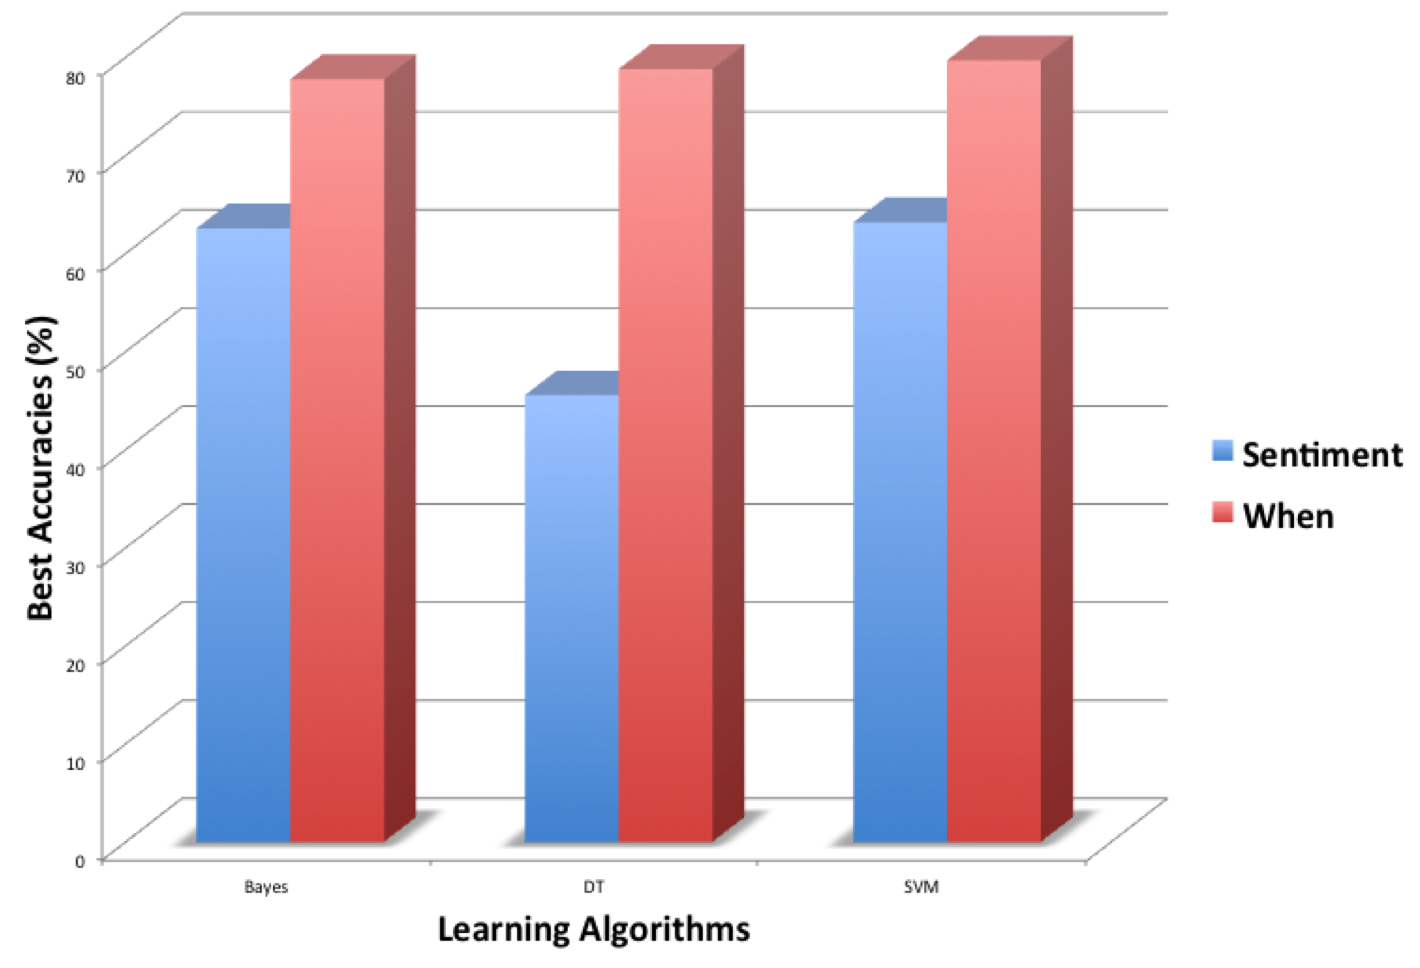
\includegraphics[width=\linewidth]{results/comparison}
  \caption{Comparison of Learning Algorithms}\label{fig:comparison}
\endminipage}
\end{figure}


	With regards to MRF, we unfortunately unable to fully implement the algorithm as specified earlier. We do, however, have a strong hunch as to what sorts of results we would have seen given the constraints of our problem. In the ideal situation, MRF would perform better than Naive Bayes, as it essentially does everything Naive Bayes can do in addition to taking account spatial/temporal dependencies. But, our formulation is not quite granular enough to expect decent accuracies. For instance, we planned to work under the assumption that the weather within each state was uniform, and the weather within one entire state is similar to that of a neighboring state. Weather varies a lot within a state, especially for large states, so we really would need to get down to the level of latitudes and longitudes (which was not available in our data set).

	Moreover, we hoped to look a small enough window of time to be able to assume that the weather within that window does not vary much. The smallest time frame we could use while still having a sufficient number of training examples was about one day -- but in practice, even one day is not small enough, because we Ithacans know better than anyone that the weather can change drastically within a day. 

	In the future, we'd like to collect more data to make this algorithm feasible, and hopefully then we can experiment with MRF and see if our high expectations are met. 
